\documentclass{bioinfo}
\copyrightyear{2017} \pubyear{2017}

\access{Advance Access Publication Date: Day Month Year}
\appnotes{Application Note}

\usepackage{url}

\begin{document}
\firstpage{1}

\subtitle{Subject Section}

\title[short Title]{Phylotyper: {\it In silico} predictor of subtypes from gene subtypes}
\author[Whiteside \textit{et~al}.]{Matthew D. Whiteside\,$^{\text{\sfb 1,}*}$, Chad R. Laing\,$^{\text{\sfb 1}}$ and Victor P.J. Gannon\,$^{\text{\sfb 1,}*}$}
\address{$^{\text{\sf 1}}$National Microbiology Laboratory, Public Health Agency of Canada, Lethbridge, AB, Canada, T1J 3Z4}

\corresp{$^\ast$To whom correspondence should be addressed.}

\history{Received on XXXXX; revised on XXXXX; accepted on XXXXX}

\editor{Associate Editor: XXXXXXX}

\abstract{\textbf{Summary:} Whole genome sequencing (WGS) is being adopted in public health for improved surveillance and outbreak analysis.
In public health, subtyping has been used to infer phenotypes and distinguish bacterial strain groups.
\textit{In silico} tools that predict molecular subtypes from sequences data are needed to transition historical data to WGS-based protocols.
Phylotyper is a novel solution for \textit{in silico} subtype prediction from gene sequences.
Designed for incorporation into WGS pipelines, it is a general prediction tool that can be applied to different subtype schemes.
Phylotyper uses phylogeny to model the evolution of the subtype and infer subtypes for unannotated sequences.
The phylogenic framework in Phylotyper improves accuracy over approaches based solely on sequence similarity and provides useful contextual feedback.\\
\textbf{Availability and Implementation:} Phylotyper is a python and R package. It is available from: \url{https://github.com/superphy/insilico-subtyping}.\\
\textbf{Contact:} \href{matthew.whiteside@phac-aspc.gc.ca}{matthew.whiteside@phac-aspc.gc.ca}\\
\textbf{Supplementary information:} Supplementary data are available at \textit{Bioinformatics}
online.}

\maketitle

\section{Introduction}

Whole-genome sequencing (WGS) is transforming the public health field by providing an efficient method for surveying bacterial populations.
The speed, discriminatory power and broad utility of WGS can improve surveillance and outbreak analysis.
Adoption of WGS in public health, however, requires transitioning of historical data with the new methods \citep{Jenkins2015}.
One of the workhorse methods in public health is subtyping.
Subtyping methods can broadly categorized as phenotype-based or DNA-based.
Phenotype-based subtypes are, for example, interrogated by biochemical tests (biotyping), detection of surface antigens (serotyping) or susceptibility to bacteriophage (phagetyping) \citep{Wiedmann2002}.
Alternatively DNA-based subtyping examines and classifies bacteria based on genetic content.
DNA-based subtypes use a variety of methods from PCR to Pulse Field Gel Electrophoresis to DNA sequencing to assign groups to bacteria \citep{Wiedmann2002}.
As a surveillance tool, subtypes provide a clearcut designation that is typically used to distinguish taxonomic groups and infer phenotypes, for example, pathogens from non-pathogens.
A WGS-based approach to subtyping would have several benefits over current subtype systems; it would be faster, have improved discrimination and would be cheaper and easier to maintain\citep{Jenkins2015}.
Accordingly, new \textit{in silico} tools have been developed to predict subtypes from WGS data \citep{Joensen2015,Ingle2016,CARRILLO2016}.
To predict from WGS data, these tools have targeted subtypes (either Phenotype-based or DNA-based systems) that can be casually linked to a specific region or gene in the genome.
\textit{In silico} subtyping has not been applied to subtyping methods that already directly use the DNA sequence to assign subtype such as Multi-Locus Sequnce Typing (MLST). 
No inference or extrapolation is needed to integrate a direct DNA sequence-based method, like MLST, into a WGS system.
An example of a subtype system that has been adpated for WGS is serotyping in \textit{Escherichia coli}.
The sequence of O-antigen processing genes in \textit{E. coli} is used to predict O-antigen group serotype in \citep{Joensen2015,Ingle2016}.
Another example, is the Shiga toxin subtype (Stx); a DNA-based subtying scheme generated using PCR.
The tool in \citep{CARRILLO2016} predicts Stx subtype by simulating PCR \textit{in silico}.

Phylotyper is a novel \textit{in silico} predictor of subtypes from sequence data.
Similar to \citep{Joensen2015,Ingle2016,CARRILLO2016}, it also works on subtypes that can be predicted from specific, pre-selected gene or genomic region sequences.
Phylotyper is unique in that it builds a phylogenetic tree consisting of reference sequences with known subtype and the unknown query sequences to help inform subtype prediction.
Using phylogenetic ancestral state reconstruction to assign the likelihood of each subtype to the tree branch points, Phylotyper then assigns an unknown query sequence a subtype based on the extrapolated value from its ancestors in the tree.


\section{Implementation}

The core of Phylotyper is an ancestral state reconstruction (ASR) method that has been adapted for hidden state prediction.
In phylogenetic analysis, ancestral state reconstruction involves the prediction of traits of ancestors from existent descendants.
This methodology can be extended to also predict properties in a limited number of existing strains.

In Phylotyper, the \texttt{rerootingMethod} function from the phytools R package is used to perform the ASR \citep{Revell2011}.
This function calculates the maximum marginal likelihood for unknown tip nodes in a phylogenetic tree.
The likelihood reflects the most likely state for the node given the empirically estimated subtype evolution model and phylogeny.
In the context of Phylotyper, the marginal likelihood provides a confidence value associated with a predicted subtype.

Phylotyper is developed in python and R. 
The steps in the Phylotyper pipeline are: 
(1) Identify subtype gene loci in input genomes using BLAST \citep{Camacho2009}. Inputs are in fasta format. Hits that do not align over 95\% or have under 90\% sequence identity with reference sequence are discarded. Users are notified if no loci are found in genome.
(2) Align input genes against a pre-aligned set of reference genes using MAFFT's \texttt{--add} feature \citep{Katoh2013}.
(3) If multiple loci are involved, concatenate individual alignments into superalignment.
(4) Generate maximum likelihood phylogenetic tree of aligned genes with FastTree \citep{Price2010}.
(5) Run phytools \texttt{rerootingMethod} using the phylogenetic tree and assigned subtypes \citep{Revell2011}.
(6) Identify the subtype with maximum marginal likelihood for the unknown genes and report to user in text output file.
Users are also provided with an image of the phylogenetic tree overlaid with the likelihood values (e.g. Figure~1\vphantom{\ref{fig:01}}).

Detailed descriptions on how to run Phylotyper and the underlying methods are provided here: \url{https://github.com/superphy/insilico-subtyping}.

\begin{figure}[!tpb]%figure1
\centerline{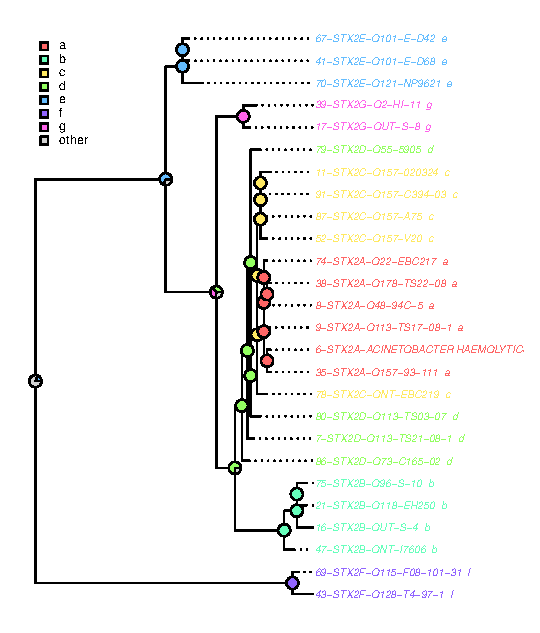
\includegraphics{fig01.eps}}
\caption{Phylogenetic tree for select Stx2 genes. 
The subtype marginal likelihood is displayed at each node as a pie chart. Subtype is indicated by color as shown in the legend. The full Stx2 tree is displayed in Supplementary Figure S1.}\label{fig:01}
\end{figure}

Phylotyper was designed to be incorporated into a WGS workflow.  
The main input into Phylotyper is assembled genome sequences (in fasta format).  
Putative loci needed for the subtype scheme are identified in the input genomes using BLAST \citep{Camacho2009}.
The identified loci are then sent to the Phylotyper subtype prediction module.
It is possible in Phylotyper to use multiple loci for subtype prediction.
Individual loci alignments are concatenated to form a single superalignment that is used to build the phylogenetic tree.

Currently, the Phylotyper package includes the following subtype schemes for \emph{Escherichia coli} (\textit{E. coli}): Stx, intimin and serotype O- and H-types  (Supplementary Table~1).
However, the Phylotyper software also has the capability to add new subtype schemes (instructions are provided here: \url{https://github.com/superphy/insilico-subtyping}). 
Creating a new subtype scheme will save the required reference files, allowing newly added schemes to be easily re-run from Phylotyper.
To add a new subtype scheme for use in Phylotyper, users require a training set of homologous sequences with assigned subtype whose phylogenetic grouping is predictive of the subtype.
Phylotyper assumes that the provided training sequences are 1) homologous, specifically, they are suitable for alignment and phylogenetic reconstruction 2) the sequence phylogeny is correlated with the subtype distribution and 3) the set is representative of the range of sequences that make up a subtype.
Where possible, checks are built-in to the \texttt{new} pipeline to validate the submitted reference set.
Specifically, each new subtype is subject to two tests in the \texttt{new} pipeline and results are reported to the user.
The first test checks that the distribution of inter-patristic phylogenetic distances between the instances of the same subtype is both smaller and distinct from non-identical subtypes.
This test can identify isolated cases of potentially mislabelled subtype genes that are tightly clustered with other subtypes.
A second check computes the accuracy measure, F-score, through a leave-one-out cross-validation; a procedure which uses each sequence in the training set as a test input to estimate positive and negative prediction rates (Supplementary Methods).
The performance metrics: recall and F-score rapidly decrease as the correlation between the training set phylogeny and subtype distribution decreases (Supplementary Figure)
These checks will verify that the training set sequences' phylogenetic grouping is predictive of the subtype.
There is no check that can confirm the training set covers all subtypes in a particular scheme; Phylotyper can only predict subtypes that are covered in the trainging set.
It is important that the user monitor and update schemes as gaps are identified.
Phylotyper is designed to return a \texttt{non-significant/undetermined} result when encountering a unknown subtype that has no representative in the training set.
Phylotyper is comparatively more robust than other methods as it generates fewer Type-I errors when encountering novel alleles or subtypes not present in the training set (see Results section for details).

\section{Results}

Phylotyper marks a progression from the sequence-similarity approach that is the basis of multiple \textit{in silico} subtyping strategies.
It's performance extends beyond allele matching, to perform accurate inference of subtypes for input gene sequences that are not in the training data or reference database.
To compare Phylotyper to a sequence similarity-based approach, we ran two validations that looked at how both methods perform when confronted with 1) gene sequence or 2) subtype class not present in the training set.
The first validation was a leave-one-out cross-validation test that iterated through each gene in the training set, retraining the prediction tools on a training set which excludes the selected test gene, and then confirming if the retrained predictor could recover the subtype of the test gene.
This validation tests how the predictors perform when run on a distinct sequence that is not in the training set.
The second validation examined how the predictors respond when presented with a gene that has a subtype not found in the reference set.
In this validation, each subtype was iterated over and all genes that are assigned the subtype were removed from the training set.
In each iteration, we recorded the number of false-positive subtype assignments when the test sequences were used as input.
The correct response for the predictors was to return a negative result, since the subtype does not exist in the training set.
For these assessments, we developed a sequence-similarity based tool that assigns putative subtypes using BLAST.
This generalized BLAST tool assigns a subtype when the top BLAST match for an unknown query gene against an annotated reference database is above a pre-selected percent identify and alignment coverage; the query is given the subtype from the top match in this case
Details for the BLAST tool and how the assessment was conducted are available in supplementary methods section.
The assessment examined the five subtype schemes available in Phylotyper: Stx1, Stx2, Eae, H-type (FliC), O-type (Wzy \& Wzx).
When tasked with assigning a novel gene sequence (i.e. one that is not in the training set) in the leave-one-out validation, Phylotyper consistently had higher precision than a top-BLAST hit approach.
The average precision in Phylotyper was 0.99 versus 0.96 in the top-BLAST hit approach(result details are available in Supplementary Table S2).
In order to achieve this level of precision, the BLAST approach often had lower recall rates; it had an average recall of 0.81 compared to 0.90 with Phylotyper
Similarily, when entire subtype classes were withheld from the training set, Phylotyper had consistenly lower false positive rates for all subtypes schemes tested; the average false positive rate in this test case was 0.11, while in the BLAST approach, the average false positive rate was 0.30.
A separate assessment for the V-typer tool; a Stx subtype predictor, was run using selected Stx gene sequences from the experimentally-verified Phylotyper training set.
The test Stx genes had sufficent surrounding DNA sequence to support \textit{in silico} PCR.
In total, 24 Stx gene sequences were tested with the V-typer tool and V-typer returned results for 7, all correct.
Phylotyper can correctly predict the subtype for all these genes.
Based on this level of recall, it appears conditions in the Stx subtype setting are challenging for simulated PCR.

All new or updated subtype schemes added in Phylotyper are subject to a leave-one-out cross-validation test.
The test is part of the \texttt{add} pipeline and is used to estimate the F-score of the subtype scheme. 
The F-score reflects that predictive capability of the subtype scheme. 
If the associated phylogeny for training set gene sequences are not correlated with the subtype distribution, this will be reflected in the F-score. 
To demonstrate this property, we randomly assigned subtypes for increasing proportions of the genes in the training set and computed the F-score with the leave-one-out validation for each proportion level.
The F-score and recall rapidly decrease as the proportion of randomly altered subtypes increases (Supplementary Figure S2).

\section{Discussion}

From assembled WGS data, Phylotyper can assign unclassifed strains a molecular subtype.
Currently the Phylotyper software offers subtyping schemes for \textit{E. coli}.
It can, however, be applied to other molecular subtype schemes and Phylotyper includes functionality to build new schemes.
Phylotyper can produce predicted subtypes from any input sequence that is strongly correlated with the subtype distribution, however, input sequences with a direct biological casual link to the subtype will have fewer cavaets; A gene sequence that is casual cannot become dissassociated from the subtype through recombination or horizontal gene transfer as a gene sequence that is merely correlated with the subtype.
Outside of \textit{E. coli}, the PCR-based capsular typing system for \textit{Haemophilus influenzae}, Neurotoxin serotyping in \textit{Clostridium botulinum} and the haemagglutinin (HA) and neuraminidase (NA) types in Influenza A virus are all examples of potential future subtype schemes that can be incorporated into Phylotyper.
We plan on expanding the Phylotyper resource by adding and updating high-quality subtype schemes for other pathogens.
We encourage users to contact us with their new subtype schemes or updates to schemes (\url{https://github.com/superphy/insilico-subtyping}).

The main strategy currently in use by other \textit{in silico} tools for predicting subtypes is to use sequence similarity to annotated loci alleles.
Query genomes or genes are matched to alleles that are attributed the subtype phenotype or are correlated with the distribution of the subtype.
For example SerotypeFinder uses BLAST to find the top matches based on sequence similarity to O-antigen processing genes for \textit{in silico} O-typing, and the flagellin genes for H-typing \textit{E. coli} genes.  
O-type and H-type are transfered from the top matches to the queries provided they are above coverage and percent identity thresholds.
This general strategy of allele matching is also applied in EcOH database, however, the EcOH can directly use unassembled sequence reads as input. The EcOH tool aligns reads to alleles linked to \textit{E. coli} O-types and H-types, and identifies the top candidates that have an alignment score above pre-defined thresholds.
Performance testing showed that Phylotyper is more robust than an approach based solely on sequence similarity.
With a strict allele matching stategy, the reference or training set make-up can be critical to performance.
When alleles or even subtypes are missing in the reference database, the sequence similarity approach more frequently generates type-I errors.
Alternatively, Phylotyper computes an empirical model of subtype evolution to predict subtypes for unclassified sequences.
By estimating the phylogenetic distribution of each subtype, Phylotyper is less likely to make type-I error when encountering a novel subtype or allele. 
The empircal testing we performed demonstrated this behavior; 
the rate of false positive classifications was significantly lower than in a sequence-similarity approach in validations where we withheld an allele or an entire subtype from the training set and used it as a test input.
V-typer takes a distinct approach; it directly simulates the \textit{in vitro} wet-lab PCR procedure used to perform Stx subtyping. 
V-typer's direct replication of a wet-lab method \textit{in silico} means it can only be applied to subtypes schemes that use PCR. 
Additionally, we found in our evaluation of Stx subtypes that it failed to generate predictions for most test cases.
From a broader methodology viewpoint, one of the benefits of the phylogenetic framework in Phylotyper, is that it provides a statistical likelihood for interpreting results.
In comparison, there is no built-in mechanism in the sequence similarity approach to quantify the level of confidence in assigning alleles a subtype.

Subtypes are mainly used as a proxy for evolutionarily-related bacterial strain groups or to infer phenotypes.
A recent analysis of O-antigen serotypes and their associated O-antigen gene sequences in \textit{E. coli} found that the sequence data indicated several changes to the nomenclature for O-groups \citep{DebRoy2016}.
There are potentially many other subtype schemes that would not be straightforward to adapt to a WGS approach.
A tool that can evaluate the ability of a genotype to predict a subtype would be better equipped for developing the new subtype schemes or updating current schemes for WGS workflows.
Phylotyper's \texttt{add} pipeline tests subtype schemes for their predictive accuracy by returning an F-score based on a cross-validation assessment.
The validation verifies that the phylogeny generated by the training set sequences can be used to predict the subtypes with a high level of accuracy.
We showed in empirical tests that the farther a subtype is dissociated from the genotype, the lower the F-score computed in the Phylotyper \texttt{add} pipeline.
In addition to this subtype-level verification, Phylotyper also computes confidence scores for each individual prediction that reflect the rate of subtype change occuring at the input gene's phylogenetic locale.
If an input sequence falls in region in the phylogenetic tree where the subtype is highly fluid due to evolution or poor subtype-genotype correlation, users would be notified in the condifidence score and in phylogenetic tree visualization output by Phylotyper. 
Phylotyper ability to inform users about the level of agreement between the subtype assignments and genotype makes it uniquely capable to transition historical subtype data to new whole genome sequence-based systems.\vspace*{-10pt}

\section*{Funding}

This work is funded in part by the Public Health Agency of Canada and a grant from the Genomics Research and Development Initiative\vspace*{-12pt}

\bibliographystyle{natbib}

\bibliography{phylotyper}


\end{document}
